\documentclass{polytech/polytech}

\typereport{prddi5}

\reportyear{2018-2019}
\title{Outil de gestion de parcours patient dans un hôpital de jour}
\student[di5]{Romain}{ROUSSEAU}{romain.rousseau@etu.univ-tours.fr}
\academicsupervisor{Yannick}{KERGOSIEN}{yannick.kergosien@univ-tours.fr}

\resume{}

\motcle{}

\abstract{}

\keyword{}

\posterblock{}{}{images/LOGO_APHP}{}

\posterblock{}{}{images/LOGO_APHP}{}

\posterblock{}{}{images/LOGO_APHP}{}


\addbibresource{PRD2.bib}

%%%%%%%%%%%%%%%%%%%%%%%%%%%%%%%%%%%%%%%%%%%%%%%%%%%%%%%%%%%%%%%%%%%%%%%%%%%%%%%%%%%%%%%%%%%%%%%%%%%
%%%%%%%%%%%%%%%%%%%%%%%%%%%%%%%%%%%%%%%%%%%%%%%%%%%%%%%%%%%%%%%%%%%%%%%%%%%%%%%%%%%%%%%%%%%%%%%%%%%

\begin{document}

\chapter*{Introduction}

Ce rapport traite du projet Recherche et Développement réalisé au sein de l'école Polytech. Il se déroule lors la cinquième année d'étude et représente une forme de synthèse des connaissances acquises lors des années d’études précédentes. Il permet de développer et d’approfondir son savoir sur un ou plusieurs champs de compétences spécifiques, afin de devenir un spécialiste du domaine choisi dans le cadre du projet. Ce travail est mené seul, sous la supervision d'un tuteur académique et, pour certains projets, avec l’aide d’un intervenant extérieur qui fait partie des initiateurs du sujet. Il permet ainsi de développer son autonomie en menant à bien un travail des prémices jusque, dans le meilleur des cas, à la production.

J'ai décidé de me consacrer à un projet lié à un enjeu important de notre société: la gestion des patients dans un hôpital. Aujourd'hui, les hôpitaux sont l'objet de nombreux débats dans l'actualité, et l'un des points de discorde majeurs concerne la gestion des patients au sein des hôpitaux. Plusieurs problèmes peuvent être cités: un temps d'attente bien trop long pour les patients (que ce soit une fois à l'hôpital ou pour avoir un rendez-vous avec un spécialiste), des problèmes de ressource (concernant le personnel ou bien les salles à disposition) ou encore des problèmes d'ordre financier en général. Certaines de ses problématiques peuvent être étudiées selon le point de vue de l'optimisation, et la recherche opérationnelle peut permettre d'améliorer certains aspects de la gestion actuelle. Pour ma part, me pencher sur les problèmes de recherche opérationnelle en général m'intéressait, et avoir l'opportunité de réaliser un projet dans ce domaine, d'autant plus dans un secteur qui en a besoin, était une bonne occasion pour améliorer mes compétences.

Le sujet de ce travail rentre dans le cadre d’un projet visant à développer un outil de gestion temps réel de parcours de patients pour l’AP-HP (Assistance publique - Hôpitaux de Paris). L'objectif de cet outil est de gérer un ensemble de patients nécessitant plusieurs activités de soins planifiées sur une journée dans un hôpital de jour. Chaque patient doit suivre un « parcours de soins » défini par un ensemble d’activités de soins. Certaines doivent être réalisées avant d'autres (contraintes de précédences) alors que pour d'autres, l’ordre n’a pas d’importance. Il peut exister des délais d'attente à respecter entre les activités. Chaque activité de soin est caractérisée par une durée et un ensemble de ressources nécessaires pour la réaliser. Ces ressources peuvent représenter le personnel, la salle où s'effectue l'activité ou encore le matériel utilisé. Elles sont caractérisées par une quantité et un horaire où elles sont disponibles. L'idée de l'outil est de pouvoir proposer un calendrier adaptatif dans lequel les horaires des activités de soins des patients peuvent être ajustés en fonction des aléas potentiels (retard, patient absent, etc.) afin de diminuer du mieux possible le temps d'attente des patients.

Ce projet est la suite de plusieurs travaux effectués à l'école ces dernières années et qui ont abouti à une première version simple d'un outil sous forme de plateforme web. L'objectif est d'améliorer l'outil actuel en corrigeant certains problèmes et en ajoutant des fonctionnalités afin de se rapprocher d'une version finale exploitable à l'avenir. Parmi les fonctionnalités qui devront être ajoutées, on peut notamment penser à la planification automatique des activités de soin sur le calendrier ou encore l'ajout de notions de temps réel sur les éléments du calendrier.

La première partie de ce rapport sera consacrée à l'analyse préliminaire de la plateforme et à la détermination des tâches à réaliser. Elle comprend des éléments sur le contexte de la réalisation, la description de la plateforme telle qu'elle se trouvait au début du projet, un état de l'art sur les outils existants et sur la gestion de la planification des activités, et la présentation des tâches qui seront effectuées durant les semaines de projet. La seconde partie sera dédiée aux détails des développements de la plateforme. Des documents complémentaires sont disponibles en annexe de ce rapport comme les diagrammes de Gantt, les diagrammes UML, des éléments de gestion de projet, etc. Un guide développeur destiné aux personnes qui désireront reprendre le projet à l'avenir est également présent en complément.


\part{Analyse préliminaire et détermination des objectifs}


Cette partie correspond à la première phase du Projet Recherche et Développement, la partie Recherche. Dans le cadre de ce projet, cette partie sera une analyse générale de la plateforme existante afin de déterminer quels objectifs nous devrons atteindre à l'issue de ce projet. Le premier chapitre sera consacré au contexte de la réalisation, la raison de l'initiation du projet ainsi que les acteurs concernés. Le chapitre suivant décrira la plateforme telle qu'elle se trouvait à la reprise du sujet, en détaillant la structure et les fonctionnalités qu'elle contient. Enfin le dernier chapitre évoquera des éléments de recherche opérationnelle dans le domaine de la gestion des patients dans un hôpital. 


\chapter{Contexte de la réalisation et objectifs}
\label{chap:contexte}

Ce chapitre présente le contexte du sujet et les objectifs à atteindre à l'issue du projet.

\section{Contexte, enjeux et acteurs}

La santé dans notre société est un sujet prédominant dans l'actualité. De nombreux débats existent concernant la modernisation des structures hospitalières et surtout, la réduction des dépenses dans le secteur. Cependant, ces problématiques sont très complexes à gérer car il est important de maintenir une certaine qualité d'accueil nécessaire au bon traitement des patients, néanmoins une baisse des dépenses pourrait se répercuter dans la qualité des prestations. L'un des aspects sur lesquels ce projet sera consacré est la gestion de prise de rendez-vous médicale. Les consultations sont soumises à de nombreux aléas, que ce soit côté patient comme côté médecin. Il n'est pas rare pour un patient de devoir attendre plusieurs mois avant d'avoir un rendez-vous chez un spécialiste, tout comme il est fréquent pour un médecin de se retrouver avec un patient absent lors d'un rendez-vous. Ceci entraîne de la frustration et du gaspillage de ressources en général. Des solutions dans le domaine de la recherche opérationnelle peuvent être mises en place, afin d'améliorer la gestion des ressources médicales et de réduire les temps d'attente pour les patients, que ce soit avant ou pendant la prise en charge. 

Les services hospitaliers sont souvent surchargés par le nombre de patients dans l'établissement. Il est de plus en plus fréquent de voir les hôpitaux proposer des services en ambulatoire, c'est-à-dire prendre en charge un patient sur une seule journée, évitant ainsi les frais pouvant s'appliquer lorsqu'un patient dort sur place. Les dépenses liées aux hospitalisations sont parmi les plus importantes dans un établissement et de nos jours, les hôpitaux proposent même des alternatives pour que les patients ne restent pas sur place la nuit, comme par exemple des chambres d'hôtel afin de ne pas occuper une chambre pendant l'hospitalisation \cite{noauthor_chu_nodate}. Un établissement, ou une partie d'établissement, proposant ce type de service est appelé "hôpital de jour".

L'idée d'implémentation d'un outil numérique dans une structure implique une réflexion sur les concepts liés l'hospitalisation d'un patient. Il est possible de définir, selon les pathologies à traiter, un parcours-patient à suivre. Un parcours-patient (ou parcours-clinique) est un plan de soins pluridisciplinaires exposant les étapes que doivent un patient pour un problème spécifique. On peut les décomposer en plusieurs activités prédéfinies, certaines devant être réalisées avant d'autres (ce qu'on appelle une contrainte de précédence), nécessitant des ressources physiques ou matérielles (contrainte de ressources) et devant être effectuées dans un délai ou un créneau horaire précis (contrainte temporelles). La mise en place d'un système de centralisation des parcours-patient reste difficile, notamment car elle repose en priorité sur une bonne communication entre les services d'un établissement. Néanmoins, cela permettrait d'avoir potentiellement une meilleure utilisation des ressources de l'hôpital et par conséquent, un effet favorable sur les durées d'hospitalisation et les dépenses hospitalières entre autres.

L'Assistance Publique - Hôpitaux de Paris (AP-HP), dans son plan stratégique 2015 - 2019, a lancé une réflexion sur la mise en place d'une clinique ambulatoire. Avec la mutualisation de certains services au sein de différents hôpitaux de la région, le site de l'hôpital \textit{Béclère}, situé dans la ville de Clamart dans le département des Hauts-de-Seine, obtiendra un gain de place suffisant pour proposer une telle solution. Il regroupera tous les hôpitaux de jour existants du site, avec un management centralisé et transversal à l'aide de parcours-patients. Les équipes médicales et administratives ont pris le soin de définir d'ors et déjà une vingtaine de parcours patients en adéquation avec les ressources déjà en place, et présenté une répartition type des prises en charge hebdomadaire. Celle-ci devrait en théorie permettre d'accueillir 179 patients chaque semaine, et à terme environ 1000 par mois. Ainsi, la conception d'un système d'aide à la décision pour la prise de rendez-vous serait utile pour une nouvelle structure comme celle-ci.

Le sujet a été proposé en 2015 par Lucie ROUSSEL, ingénieur en ordonnancement à l'AP-HP et a été suivi lors de plusieurs projets à Polytech: tout d'abord, lors d'un projet collectif (réalisé par les étudiants Benjamin COLMART, Jean COQUELET, Anaëlle HAMON, Jiang MING, Yan LI et Minghui ZHANG) qui a posé les bases de la modélisation et des premières fonctionnalités, un projet R\&D effectué par Jean COQUELET en 2016 également basé davantage sur l'aspect gestion et optimisation des parcours, un projet R\&D par Guillaume POCHET en 2017 qui a ajouté des éléments sur la gestion de calendrier et enfin un autre projet R\&D réalisé par Jing YANG qui ajoute des améliorations générales. Le projet tel qu'il est développé à Polytech servira dans un premier temps en tant que \textit{proof of concept}, et si celui-ci satisfait l'administration, il pourra entrer en production à plus grande échelle dans le futur.

La plateforme, une fois installée sur mon poste à la reprise du projet, fonctionne. Il est possible d'ajouter des patients et de leur associer un parcours-patient avec des heures de rendez-vous et des activités à suivre lors d'une journée. Cependant, de nombreux éléments sont à améliorer, des bugs à corriger dans un premier temps mais aussi des améliorations d'un point de vue graphique. Des fonctionnalités importantes restent à implémenter: d'un côté, l'ajout d'une notion de temps réel sur les activités et les rendez-vous, et de l'autre, la possibilité de faire une planification automatique tenant compte des patients et des ressources disponibles. Compte-tenu du temps alloué pour le projet, il sera difficile d'ajouter ces deux fonctionnalités importantes. Nous verrons par la suite vers quels éléments nous allons nous pencher en priorité. 


\section{Objectifs}

Suite à l'affectation du sujet, les premières rencontres avec M. KERGOSIEN ont permis de fixer des objectifs principaux pour mener à bien le projet. Trois axes de développement ont été définis pour la finalisation de la plateforme : la correction de certains problèmes sur les fonctionnalités existantes, l'ajout de fonctions de planification automatique et l'implémentation de fonctionnalités permettant de planifier en temps réel. 

Les trois objectifs présentés par la suite sont conséquents en terme de temps. Il sera sans doute très compliqué de réaliser les trois objectifs dans la limite de temps alloué au projet. Nous nous focaliserons ainsi sur deux des trois objectifs à suivre. 


\subsection{Corrections des bugs et améliorations sur les fonctionnalités existantes}

Le premier objectif consiste à corriger certaines erreurs que l'on peut trouver sur la plateforme. À la première analyse du projet, plusieurs problèmes sont apparus, que ce soit des erreurs d'affichage ou des soucis d'ergonomie par exemple. Ainsi, le but est d'améliorer les éléments déjà existants de la plateforme afin de la rendre plus stable et de meilleur qualité. Parmi les corrections et améliorations à apporter, on retrouve la révision de la suppression de données, de l'onglet "Plan de parcours", du formulaire de création de patient, de certains éléments de la page d'accueil. 

Plusieurs fonctionnalités qui n'ont pas encore été implémentées sont aussi à rajouter pour enrichir les possibilités offertes à l'utilisateur, comme l'affichage du planning pour un patient donné, l'ajout de fonctions de tri pour l'affichage des ressources, ou encore, la création de jeux de données permettant de tester plus facilement la planification. 


\subsection{Implémentation de la planification automatique}

L'une des parties principales du projet consiste à l'élaboration de la planification automatique les rendez-vous médicaux. À l'heure actuelle, la planification des rendez-vous se fait de façon manuelle. Une fois les patients définis pour une journée, un calendrier et la liste des activités à réaliser sont à disposition. Par un système de "glisser-déposer", l'administrateur peut agencer les activités selon les ressources disponibles (en terme de personnels ou de matériels). Cependant, l'agencement manuel des activités peut prendre un temps considérable, car pour chaque activité, il faut prendre en compte les activités qui peuvent la précéder ou la suivre, voir si le personnel est disponible, si les salles le sont également, etc. Lorsque le nombre de patients commence à se multiplier, la planification manuelle des activités devient un véritable casse-tête.

La planification automatique des activités permettrait d'avoir un premier agencement plus facile, et par conséquent, de gagner un temps considérable lors de l'élaboration des plannings. La notion d'automatisme peut être néanmoins très large, il sera important de la définir. Cela peut aller de la planification la plus simple, sans prendre en compte certaines contraintes et que l'utilisateur pourra corriger à sa guise, à une planification complète avec des options sélectionnées (agencement des activités au plus tôt de la journée, minimisation du temps d'attente pour les patients, pour les médecins, etc.). Une donnée importante est à prendre en compte: plus le type d'automatisation que l'on souhaite est précise ou détaillée, plus la modélisation nécessaire pour trouver une solution sera complexe. Ainsi, le but sera dans un premier temps de réaliser une première automatisation la plus simple possible puis, si les conditions sont réunies, faire évoluer le modèle et le complexifier davantage.


\subsection{Implémentation de la planification temps réel}

Le dernier objectif fixé lors des premières réunions est l'ajout d'une notion de temps réel à l'application. La plateforme pour le moment est conçue pour que l'utilisateur crée un planning pour une journée à un moment particulier (le matin avant les consultations ou le soir pour les rendez-vous du lendemain). Une fois le planning acté, il est difficile de le modifier en direct si un aléa se produit (par exemple, si un rendez-vous est annulé) à cause notamment des contraintes de précedence et de durée qui peuvent exister entre les activités. 

L'idée serait donc d'ajouter des fonctionnalités permettant d'ajuster le planning en temps réel. Tout comme la planification automatique, cela peut impliquer des concepts différents qu'il est nécessaire de définir. Cela peut aller d'un simple indicateur sur le calendrier pour voir où nous en sommes dans la journée, jusqu'à un système de pointage pour chaque activité. Il est possible d'imaginer un outil pour lequel les médecins pointent à chaque début de rendez-vous puis signalent dès que le rendez-vous est terminé sur la plateforme. Ainsi, il serait possible d'ajuster les activités en temps réel en cas de retard voire même en cas d'avance sur la planning. 

Se pencher sur la planification en temps réel nécessiterait une refonte de la modélisation du système, notamment en ce qui concerne les activités. Compte tenu du temps alloué au projet et aux autres objectifs à réaliser, nous avons décidé de nous focaliser en priorité sur les deux premiers objectifs. Si les évolutions avancent plus rapidement que prévu, nous pourrons songer à implémenter certains éléments. Dans un premier temps, nous nous tiendrons au chiffrage initial du projet (chiffrage disponible en \autoref{ann:chiffrage}).


\section{Bases méthodologiques}

À l'issue des premières réunions de lancement du projet, nous avons avec mon encadrant établi un chiffrage du projet avec les objectifs à réaliser et une estimation du temps de travail pour chaque activité. Ce chiffrage est visible en \autoref{ann:chiffrage}. Une fois le chiffrage effectué, j'ai établi un diagramme de Gantt pour planifier les étapes au long du projet. Le découpage des étapes peut s'apparenter à une méthode Agile, avec un sprint représentant une étape à réaliser. Les détails concernant le découpage et le cheminement du projet sont disponibles en \autoref{ann:gantt}.

En ce qui concerne l'organisation des tâches, j'utilise l'outil de gestion de projet \textit{Trello}. Les détails concernant l'outil et l'utilisation que j'en ai fait sont disponibles en \autoref{ann:gestion}.

Concernant la méthodologie de développement, la plateforme a été réalisée en suivant un pattern MVC. Je vais donc reprendre le code en respectant l'organisation déjà établie.


\chapter{Description générale}


Ce chapitre est consacré à la description générale de la plateforme. Nous évoquerons l'environnement autour du projet, les caractéristiques des futurs utilisateurs, les fonctionnalités du système ainsi que sa structure générale.

\section{Environnement du projet}


Comme évoqué dans le \autoref{chap:contexte}, ce projet est la reprise de plusieurs projets successifs effectués par les étudiants de Polytech. Il a été initié lors de l'année scolaire 2015-2016 avec un projet R\&D et un projet collectif en simultané. Par la suite, plusieurs projets R\&D se sont imbriqués chaque année de façon successive. La première modélisation et les premières briques de code datent donc de plusieurs années maintenant. 

L'application existante fonctionne sur une machine locale et est déployée via la plateforme de développement Web WAMP. Cette plateforme permet de faire fonctionner localement des scripts PHP sur machine Windows. WAMP fait le lien entre 4 composantes comme indiqué dans son acronyme : 

\begin{description}
	\item[Windows] comme le nom du système d'exploitation qui assurera la distribution des ressources entre les composants;
	\item[Apache] comme le serveur Web qui va déployer l'application et répondre aux requêtes Web du navigateur;
	\item[MySQL] comme le nom de la base de données utilisée pour l'application;
	\item[PHP] comme le langage de script utilisé. 
\end{description}

Les développements lors de ce projet ont été effectués sur ma machine personnelle, sous Windows 10, et en utilisant le navigateur \textit{Mozilla Firefox}. Le diagramme de déploiement de la \autoref{fig:deploiement} représente les liens entre le serveur, la base de données et l'application. 

\begin{figure}
	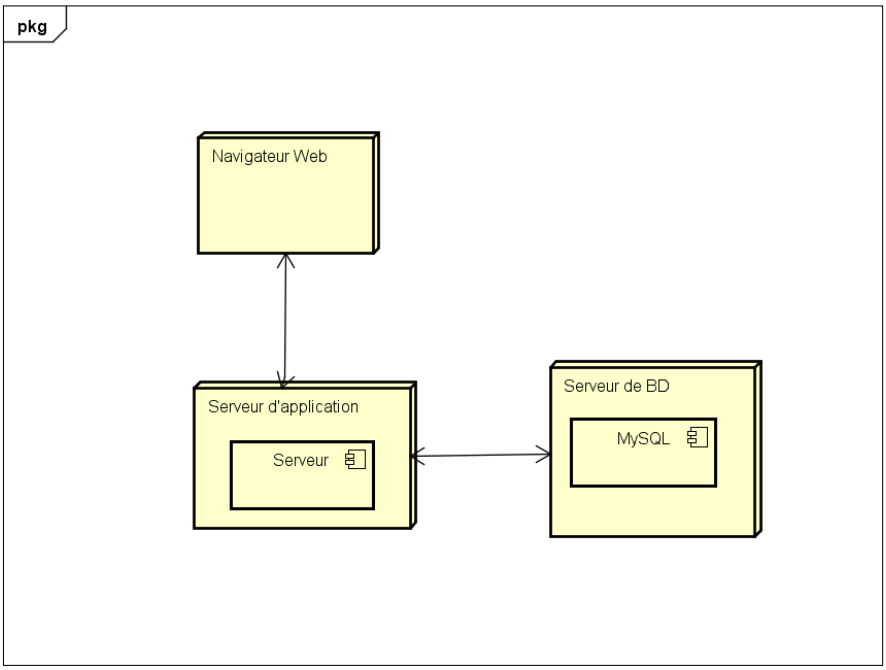
\includegraphics[scale=0.8]{images/deploiement}
	\caption{Diagramme de déploiement}
	\label{fig:deploiement}
\end{figure}

L'application si elle est mise en production sera disponible dans un premier temps sur une machine à la disposition de la personne chargée de la coordination du planning au sein du service. Les évolutions sur la plateforme pourront amener à déployer l'application sur plusieurs machines en parallèle au sein de l'hôpital. Par exemple, si l'on souhaite implémenter un système de pointage en temps réel des activités, il serait intéressant d'avoir plusieurs postes à disposition pour faciliter la tâche. Ici, nous nous focaliserons sur un déploiement sur une unique machine. 


\section{Caractéristiques des utilisateurs}

La plateforme incorpore un système de gestion de compte afin de garantir la sécurité des données. Nous pouvons définir 2 types d'utilisateurs pour l'application.

\begin{itemize}
	\item Le personnel de soins : ils auront accès à la majorité des fonctionnalités de la plateforme (l'ajout et la recherche de patients, l'accès à leur planning personnel et au planning des patients). Ils ne pourront pas effectuer de modification sur les rendez-vous ou sur le planning en général.
	\item Administrateurs et infirmières de coordination : ils disposeront de tous les droits sur l'application. Ils pourront réaliser les mêmes opérations que le personnel de soins et auront la possibilité de gérer les ressources, gérer les activités, créer et modifier les plannings, ajouter et modifier un parcours-patient, etc.
\end{itemize}

Les utilisateurs de l'application devront s'authentifier pour pouvoir accéder aux différentes fonctionnalités et selon leur grade, ils auront accès aux éléments avec lesquels ils pourront interagir. 


\section{Contraintes de développement}

\'{E}tant donné que ce projet fait suite à plusieurs projets consécutifs et que la base de la plateforme a déjà été développée, il faudra utiliser les mêmes langages de programmes ainsi que les mêmes frameworks que lors des projets passés. Ainsi, les contraintes concernent les langages \textit{HTML}, \textit{CSS}, \textit{Javascript}, \textit{PHP}. La structure de l'application sera la même, à savoir une architecture MVC (Modèle - Vue - Contrôleur), mise en place à l'aide du framework PHP \textit{CodeIgniter}. En ce qui concerne la mise en page (\textit{CSS}), nous devrons utiliser \textit{Bootstrap}.

Guillaume POCHET, qui a effectué son PR\&D sur le sujet lors de l'année scolaire 2016-2017, avait réalisé un état de l'art sur les bibliothèques utilisables pour réaliser interactif \cite{pochet_outil_nodate}. À la suite de cela, il avait décidé d'utiliser la bibliothèque \textit{FullCalendar} pour constituer les planning sur la plateforme. Nous poursuivrons avec l'utilisation de cette même bibliothèque.


\section{Fonctionnalités du système}


Les fonctionnalités existantes sont dispo en annexe.



\section{Structure générale du système}


\chapter{État de l'art}


\section{Planification automatique}


\part{Développement}


\chapter{Analyse et conception}


\chapter{Mise en œuvre}


\chapter{Bilan et conclusion}


\appendix

\chapter{Fonctionnalités existantes}



\chapter{Explications des tables du modèle}


%%PRD Jing

Voici l'explication sur les tables créées dans l'ancien projet [2]que je vais continuer à utiliser.

\begin{description}
	\item[Activité] : Table regroupant l'ensemble des informations concernant une activité. C'est cet élément qui constitue les parcours. Une activité peut obliger la réalisation de certaines autres activités avant d'être réalisable. Cette notion de dépendance dépend du parcours en cours. Cette notion de précédence est sera vue plus loin via la table composer. En plus de cela, une activité a besoin de ressources. Ce lien se fait par la table nécessiter.
	\item[Champ] : Table contenant l'ensemble des champs qu'il est possible d'ajouter dans un onglet d'un dossier Parcours. À chaque champ est lié un type de champ, que nous verrons plus loin, avec la table typechamp.
	\item[Composer] : Table permettant de faire le lien entre un parcours et une activité. Par l'intermédiaire de cette table nous pouvons dire en fonction d'un parcours et d'une activité s'il y a des besoins en termes de précédence. Chaque ligne, dans cette table, a pour signification : « Pour l'activité A dans le parcours P, il faut avoir réalisé l'activité B avant, et ce dans un délai compris entre delaiMin et delaiMax. ». Il est important de noter qu'il est possible de mettre à « null », l'id de l'activité précédente.
	\item[Compte] : Table regroupant l'ensemble des comptes qu'ils soient des comptes patient ou des comptes de type ressource médicale.
	\item[Constituerdossier] : Table permettant de faire le lien entre un dossier parcours et les informations qui le constituent. En effet, nous retrouvons pour chaque dossier parcours et pour chaque onglet dans ce dernier, la valeur des champs le composant.
	\item[Dossiergenerique] : Table définissant, pour un parcours, les onglets et les champs que tous les dossiers parcours doivent avoir impérativement.
	\item[Dossierparcours] : Table renseignant les informations génériques d'un dossier parcours. Soit le patient associé, le parcours, dates de création et de dernière modification.
	\item[Etreindisponible] : Table regroupant l'ensemble des indisponibilités pour une ressource. Cette indisponibilité est caractérisée par une date de début et de fin, acceptant toutes les deux le renseignement de l'heure.
	\item[Jour] : Table qui contient les jours de semaine, ainsi que leurs index sous MySQL. Cette table a un enjeu au niveau des prévisions du nombre de patient par jour pour un parcours.
	\item[Necessiter] : Table permettant de renseigner les types de ressources requises pour une activité, ainsi que la quantité nécessaire.
	\item[Onglet] : Table des onglets disponibles pour constituer un dossier parcours.
	\item[Parcours]	 : Table décrivant un parcours de façon générale.
	\item[Personnel] : Table contenant l'ensemble de personnel médical de l'établissement. Chaque personnel a un compte, et est considéré comme une ressource.
	\item[Planparcours] : Table regroupant l'ensemble des objectifs concernant le nombre de patients pour un parcours pour un jour donné.
	\item[Ressource] : Table faisant le lien entre la table typeressource et personnel ou matériel. Ce lien	sera expliqué plus en détail avec la table typeressource.
	\item[Typechamp] : Table regroupant les différents type de champs qu'il est possible d'ajouter dans un dossier parcours. Elle contient également le code HTML des composants, permettant ainsi une	mise en page en accord avec les autres éléments des pages.
	\item[Typecompte] : Table utilisée pour la gestion des droits.
	\item[Typeressource] : Table contenant les types de ressource d'un point de vue activité. En effet, une activité peut avoir besoin d'un type de ressource bien caractéristique (ex : IDE obésité). C'est pourquoi nous avons un double niveau de type de ressource. Un concernant les activités (typeressource) et un second plus d’un point de vue logique générale (personnel, matériel).
	\item[Ordonnancer] : Table de fait de notre système. C'est la table la plus importante. Chaque ligne veut dire : « Pour le patient P qui fait le parcours Pa à la date D, il a besoin de la ressource R pour faire l’activité A de start à end. Cette table contient la planification réalisée de manière manuelle ou automatique (pas implémenté pour le moment).
	\item[Evènement] : Table identique à la table Ordonnancer. Elle a le même but que la table ordonnancer mais cette table contient la planification en cours. Cette table permet de donc de pouvoir sauvegarder ou restaurer la planification en fonction des modifications que l’utilisateur a effectuées.
\end{description}


\chapter{Chiffrage du projet}
\label{ann:chiffrage}

Revoir la suppression : 1 j
Revoir l'onglet "Plan de parcours" : 1,5 j
Revoir le formulaire de création de patient : 2 j
Revoir la page d'accueil : 1 j
Affichage du planning patient : 5 j
Ajouter des tris dans les onglets d'affichage : 1 j
Corriger le problème des URL : 2 j
Affichage des ressources sélectionnées et test planning : 10 j
Planification automatique : 20 j
Jeux de données : 3 j
Rapport : 15 j
Préparation soutenance : 3 j

\chapter{Diagramme de Gantt}
\label{ann:gantt}

\chapter{Gestion de projet}
\label{ann:gestion}

\chapter{Manuel développeur}


%TODO Supprimer le chapitre une fois terminé
\chapter{TEMPO}

\section*{Suppression}

La fonctionnalité "Supprimer" a été ajoutée lors du dernier PR\&D réalisé par Yang Jing. Elle est implémentée dans les onglets de Gestion de la plateforme pour avoir la possibilité de supprimer les ressources qui ne sont pas nécessaires ou qui sont devenues obsolètes.  

Cette fonctionnalité a des risques importants. En effet, la suppression d'un élément peut entraîner des répercussions sur l'intégralité de la plateforme (exemple ...). 

À l'heure actuelle, les boutons "Supprimer" ne disposent d'aucune sécurité, ce qui peut se révéler très dangereux. Un simple clic sur le bouton entraîne la disparition de la ressource sélectionnée. Compte tenu de la dangerosité de la manœuvre sur le bon fonctionnement de la plateforme, il est nécessaire de corriger ce problème. 

À minima, l'apparition d'un message de confirmation lors du clic sur le bouton permettrait d'éviter les mauvaises manipulations. 

Pour afficher un message de confirmation, il suffit d'ajouter \javacode{onclick="return confirm('Etes vous sur ?');"} sur le lien de l'action ...


\end{document}
